\begin{problem}[Munkres \S20, Ex.\,4(a)]
Consider the product, uniform, and box topologies on
$\RR^\omega$.
\begin{enumerate}[noitemsep]
\item[(a)] In which topologies are the following functions from
  $\RR$ to $\RR^\omega$ continuous?
  \begin{align*}
    f(t)&=(t,2t,3t,...)\\
    g(t)&=(t,t,t,...)\\
    h(t)&=\left(t,\tfrac{1}{2}t,\tfrac{1}{3}t,...\right).
  \end{align*}
\end{enumerate}
\end{problem}
\begin{proof}
The maps $f$, $g$ and $h$ are, evidently, continuous by Theorem
19.6 and the following lemmas (they may be useful in the future
so we prove them here):
\begin{lemma}[Munkres \S18, Ex.\,1]
Let $(X,d_X)$ and $(Y,d_Y)$ be metric spaces. Suppose $f\colon
X\to Y$ is continuous in $\epsilon$-$\delta$ sense. Then $f$ is
continuous in the open set sense.
\end{lemma}
\begin{proof}
\renewcommand\qedsymbol{$\clubsuit$}
Suppose $f$ is continuous in the $\epsilon$-$\delta$ sense, that
is, for every $\epsilon>0$ there exists $\delta>0$ such that
$d_X\left(x_0,x\right)<\delta$ implies
$d_Y\left(f(x_0),f(x)\right)<\epsilon$. Now, let $U$ be an open
set in $\RR$ and let $x_0\in f^{-1}(U)$. Since $U$ is open, there
exists a real number $\epsilon>0$ such that
$B_{d_Y}\left(f(x_0),\epsilon\right)\subset U$. Since $f$ is
$\epsilon$-$\delta$ continuous, there exists $\delta>0$ such that
$x\in B_{d_X}\left(x_0,\delta\right)$ implies
$f(x)\in B_{d_Y}\left(f(x_0),\epsilon\right)$ so
$B_{d_X}\left(x_0,\delta\right)\subset f^{-1}(U)$ (this is
because if $x\in B_{d_X}\left(x_0,\delta\right)$, then $f(x)\in
B_{d_Y}\left(f(x_0),\epsilon\right)\subset U$ so $f(x)\in
U$ and in particular $x\in f^{-1}(U)$). Since $x_0$ was arbitrary,
we conclude that $f^{-1}(U)$ is open.
\end{proof}
\begin{lemma}
Suppose $f,g\colon\RR\to\RR$ are continuous. Then the following
hold
\begin{enumerate}[noitemsep,label=(\roman*)]
\item The sum $(f+g)(x)=f(x)+g(x)$ is continuous.
\item The product $fg(x)=f(x)g(x)$ is continuous.
\end{enumerate}
\end{lemma}
\begin{proof}
\renewcommand\qedsymbol{$\clubsuit$}
By Lemma 8, it suffices to show that $f+g$ and $fg$ are
continuous in the $\epsilon$-$\delta$ sense: Let $x_0\in\RR$ and
let $\epsilon>0$ be given.
\\\\
(i) Since $f$ and $g$ are continuous in the $\epsilon$-$\delta$
sense there exists $\delta_1>0$ and $\delta_2>0$ such that
$|x_0-x|<\delta_1$ implies $\left|f(x_0)-f(x)\right|<\epsilon/2$
and $|x_0-x|<\delta_2$ implies $\left|g(x_0)-g(x)\right|<\epsilon/2$
respectively. Take
$\delta=\min\left\{\delta_1,\delta_2\right\}$. Then, by the
triangle inequality (cf.\,Munkres \S20 the definition of a metric
in p.\,119) we have
\begin{align*}
\left|(f+g)(x_0)-(f+g)(x)\right|
&=\left|f(x_0)+g(x_0)-f(x)-g(x)\right|
\\
&=\left|f(x_0)-f(x)+g(x_0)-g(x)\right|
\\
&\leq
\left|f(x_0)-f(x)\right|+\left|g(x_0)-g(x)\right|\\
&\leq \epsilon
\end{align*}
\\\\
(ii) Since $f$ and $g$ are continuous in the $\epsilon$-$\delta$
sense, by the triangle inequality we have
\begin{align*}
\left|fg(x_0)-fg(x)\right|
&=\left|f(x_0)g(x_0)-f(x)g(x)\right|
\\
&=\left|f(x_0)g(x_0)-f(x_0)g(x)+f(x_0)g(x)-f(x)g(x)\right|\\
&=\left|f(x_0)g(x_0)-f(x_0)g(x)\right|
+\left|f(x_0)g(x)-f(x)g(x)\right|\\
&=
\left|f(x_0)\right|
\left|g(x_0)-g(x)\right|
+\left|f(x_0)-f(x)\right|
\left|g(x)\right|.
\end{align*}
To bound this expression, consider the following: Let
$\delta_1>0$ such that
$\left|f(x_0)-f(x)\right|<\epsilon/2$. Since $g$ is continuous,
choose $\delta_2>0$ such that $\left|g(x_0)-g(x)\right|<1$. Then
$g(x)<g(x_0)+1$ for all $x\in(x_0-\delta,x_0+\delta)$. Finally,
if choose $\delta_3>0$ such that
$\left|g(x_0)-g(x)\right|<\epsilon/2f(x_0)$. Then
$\delta=\min\left\{\delta_1,\delta_2,\delta_3\right\}$ gives a
bound to the expression
\[
\left|f(x_0)\right|
\left|g(x_0)-g(x)\right|
+\left|f(x_0)-f(x)\right|
\left|g(x)\right|
<\epsilon.
\]
Note that if $f(x_0)=0$, we discard $\delta_3$ and we obtain a
stricter bound on our estimates. In any case, $fg$ is
continuous.
\end{proof}
\begin{corollary*}
Polynomials from $\RR$ to $\RR$ are continuous.
\end{corollary*}
\begin{proof}[Proof of Corollary]
\renewcommand\qedsymbol{$\clubsuit$}
It is immediate from Lemma 9(i,ii) and Theorem 18.2(a,b) from
Munkres. Here is a sketch: By Theorem 18.2(a) constant functions
are continuous, therefore $x\mapsto a_0$ for $a_0\in\RR$ is
continuous. By Theorem 18.2(b), the map $x\mapsto x$ is
continuous so by Lemma 9(ii), $x\mapsto x^2$ is continuous. By
induction on $n$, $x\mapsto x^n$ is continuous. Similarly, we
have that $x\mapsto a_nx^n$ is continuous. Thus, by Lemma 9(i),
the map
\[
x\longmapsto a_nx^n+\cdots+a_1x+a_0
\]
is continuous.
\end{proof}
Now, for the box topology, consider our favorite neighborhood of
$\mathbf{0}$ (as seen in Munkres \S19, p.\,117) given by
\[
U=\prod_{n\in\ZZ_+}\left(-\frac{1}{n},\frac{1}{n}\right).
\]
The set $U$ is clearly open since it is a basis element, by
Theorem 19.2. However, the preimage
\[
h^{-1}(U)=\bigcap_{n\in\ZZ_+}\left(-\frac{1}{n},\frac{1}{n}\right)=\{0\}
\]
is not open in $\RR$ so $h$ is not open in $\RR^\omega$ with the
box topology.

Finally, we will show that $h$ is continuous in the
$\epsilon$-$\delta$ sense: Given $\epsilon>0$ and $x_0\in\RR$,
let $\delta=\epsilon$, then for any
$x\in(x_0-\epsilon,x_0+\epsilon)$ we have
\[
d_{\bar\rho}\left(h(x_0),h(x)\right)
=|x_0-x|<\epsilon.
\]
Thus, since $h$ is continuous in the $\epsilon$-$\delta$ sense,
by Lemma 8, we have that $h$ is continuous in the open set sense.
\end{proof}
\newpage
\begin{problem}[Munkres \S20, Ex.\,4(b)]
Consider the product, uniform, and box topologies on
$\RR^\omega$.
\begin{enumerate}[noitemsep]
\item[(b)] In which topologies do the following sequences
  converge?
\begin{align*}
\mathbf{w}_1&=(1,1,1,1,...),&\mathbf{x}_1&=(1,1,1,1,...),\\
\mathbf{w}_2&=(0,2,2,2,...),&\mathbf{x}_2&=\left(0,\tfrac{1}{2},\tfrac{1}{2},\tfrac{1}{2},...\right),\\
\mathbf{w}_3&=(0,0,3,3,...),&\mathbf{x}_3&=\left(0,0,\tfrac{1}{3},\tfrac{1}{3},...\right),\\
&\vdotswithin{=}&&\vdotswithin{=}\\
\mathbf{y}_1&=(1,0,0,0,...)&\mathbf{z}_1&=(1,1,0,0,...),\\
\mathbf{y}_2&=\left(\tfrac{1}{2},\tfrac{1}{2},0,0,...\right)&\mathbf{z}_2&=\left(\tfrac{1}{2},\tfrac{1}{2},0,0,...\right),\\
\mathbf{y}_3&=\left(\tfrac{1}{3},\tfrac{1}{3},\tfrac{1}{3},0,...\right)&\mathbf{z}_3&=\left(\tfrac{1}{3},\tfrac{1}{3},0,0,...\right),\\
&\vdotswithin{=}&&\vdotswithin{=}
\end{align*}
\end{enumerate}
\end{problem}
\begin{proof}
By Lemma D (from Prof.\,McClure's notes) if
$\left\{\mathbf{x}_n\right\}$, $\left\{\mathbf{y}_n\right\}$ and
$\left\{\mathbf{z}_n\right\}$ converge in the box topology, they
converge to $\mathbf{0}$ since they converge to $\mathbf{0}$ in
the product topology (and this can be readily seen by applying
Problem 3.5 [Munkres \S19, Ex.\,6]).

However, for the sequences $\left\{\mathbf{x}_n\right\}$ and
$\left\{\mathbf{y}_n\right\}$ we see that the neighborhood of
$\mathbf{0}$ given by
\[
U=\prod_{n\in\ZZ_+}\left(-\frac{1}{n},\frac{1}{n}\right)
\]
does not contain any term of either sequence since for any
$k\in\ZZ_+$, the term
\[
\mathbf{x}_k
=\left(0,0,...,1/k,1/k,...\right)
\notin
(-1,1)
\times
\cdots
\times
\left(-1/k,1/k\right)
\times
\left(-1/(k-1),1/(k-1)\right)
\times\cdots.
\]
Similarly, we can see that $\mathbf{y}_k$ will not be in $U$ for
any $k$ so the sequence $\left\{\mathbf{x}_n\right\}$ and
$\left\{\mathbf{y}_n\right\}$ will not converge in the box
topology.

Although $\left\{\mathbf{x}_n\right\}$ and
$\left\{\mathbf{y}_n\right\}$ do not converge in the box topology
we claim that the sequence $\left\{\mathbf{z}_n\right\}$ does
converge. To see this it is enough to consider basic open
neighborhoods of $\mathbf{0}$. Let $U=\prod (a_n,b_n)$ be a basis
element containing $\mathbf{0}$. Then we must show that for $N$
sufficiently big, $\mathbf{x}_n\in U$ for all $n\geq N$. Let
$b=\min\{b_1,b_2\}$. Since $b>0$, by the Archimedean property
(Munkres Theorem 4.2), there exists $N\in\ZZ_+$ such that
$1/N<b$. Thus, $\mathbf{z}_n\in U$ for all $n\geq N$ so
$\mathbf{z}_n\to\mathbf{0}$ in the box topology.
\end{proof}
\newpage
\begin{problem}[Munkres \S20, Ex.\,6(b)]
Let $\bar\rho$ be the uniform metric on $\RR^\omega$. Given
$\mathbf{x}=\left(x_1,x_2,x_3,...\right)\in\RR^\omega$ and given
$0<\epsilon<1$, let
\[
U(\mathbf{x},\epsilon)=
\left(x_1-\epsilon,x_1+\epsilon\right)\times\cdots\times
\left(x_n-\epsilon,x_n+\epsilon\right)\times\cdots.
\]
\begin{enumerate}[noitemsep]
\item[(b)] Show that $U(\mathbf{x},\epsilon)$ is not even open in the
  uniform topology.
\end{enumerate}
\end{problem}
\begin{proof}[Proof of (b)]
It is sufficient to find a point $\mathbf{x}_0\in
U(\mathbf{x},\epsilon)$ such that
$B_{\bar\rho}\left(\mathbf{x}_0,\delta\right)\nsubset
U(\mathbf{x},\epsilon)$ for any $\delta>0$. Let $\mathbf{x}_0$ be
the point
\[
\mathbf{x}_0=\prod_{n\in\ZZ_+}\left(x_n+\left(\frac{n-1}{n}\right)\epsilon\right).
\]
Now consider the open ball
$B_{\bar\rho}\left(\mathbf{x}_0,\delta\right)$ for
$\delta>0$. Now, pick a point $\mathbf{y}\in
B_{\bar\rho}\left(\mathbf{x}_0,\delta\right)$ given by
\[
\mathbf{y}=\prod_{n\in\ZZ_+}
\left(x_n+\left(\frac{n-1}{n}\right)\epsilon+\frac{\delta}{2}\right).
\]
Clearly $\mathbf{y}\in
B_{\bar\rho}\left(\mathbf{x}_0,\delta\right)$ since
\[
\bar\rho\left(\mathbf{x}_0,\mathbf{y}\right)
=\sup_{n\in\ZZ_+}\left\{\min\left\{\left|x_n-y_n\right|,1\right\}\right\}
=\min\left\{\delta/2,1\right\}
\leq\delta/2.
\]
However, by the Archimedean property, there exists $k\in\ZZ_+$
such that $\delta/2>1/k$ so $n\geq k$ implies
\[y_n=x_n+\left(\frac{n-1}{n}\right)\epsilon+\frac{\delta}{2}>x_n+\epsilon\]
so $\mathbf{y}$ is in $B_{\bar\rho}(\mathbf{x}_0,\delta)$ but not
in $U(\mathbf{x},\epsilon)$. Since $\delta$ was arbitrary, we
conclude that $U(\mathbf{x},\epsilon)$ is not open.
\end{proof}
\newpage
\begin{problem}[A]
Prove Theorem Q.2 from the notes on Quotient Spaces.
\end{problem}
\begin{proof}
Recall the statement of the theorem:
\begin{theorem*}[Theorem Q.2]
A function $f\colon X/{\sim}\to Y$ is continuous if and only if
the composite
\[
X\overset{q}{\longrightarrow}X/{\sim}\overset{f}{\longrightarrow}Y
\]
is continuous.
\end{theorem*}
The direction $\implies$ follows from Theorem 18.2(c) in Munkres.

$\impliedby$ Suppose that the composite
\[
X\overset{q}{\longrightarrow}X/{\sim}\overset{f}{\longrightarrow}Y
\]
is continuous. Then for every open set $U\subset Y$, the preimage
$(f\circ q)^{-1}(U)$ is open in $X$. But the preimage
\[
(f\circ q)^{1}(U)=q^{-1}\left(f^{-1}(U)\right)
\]
and since $q$ is a quotient map by definition (cf.\,Munkres \S22,
p.\,137) $f^{-1}(U)$ is open in $X/{\sim}$ if and only if
$q^{-1}\left(f^{-1}(U)\right)$ is open in $X$. Thus, the map
$f\colon X/{\sim}\to Y$ is continuous.
\end{proof}
\newpage
\begin{problem}[B]
Prove Proposition Q.5 from the notes on Quotient Spaces.
\end{problem}
\begin{proof}
Recall the definition and the proposition:
\begin{definition*}
Let $X$ and $Y$ be topological spaces. A map $p\colon X\to Y$ is
a \emph{Munkres quotient map} if $\bar p\colon X/{\sim_p}\to Y$
is a homeomorphism.
\end{definition*}
\begin{proposition*}[Proposition Q.5]
A map $p\colon X\to Y$ satisfies Definition Q.4 if and only if it
satisfies the definition at the top of page 137 in Munkres.
\end{proposition*}
and Munkres's definition:
\begin{definition*}[Munkres \S22, p.\,137]
Let $X$ and $Y$ be topological spaces; let $p\colon X\to Y$ be a
surjective map. The map $p$ is said to be a \emph{quotient map}
provided a subset $U$ of $Y$ is open in $Y$ if and only if
$p^{-1}(U)$ is open in $X$.
\end{definition*}
$\implies$ Now, suppose that $\bar p\colon X/{\sim_p}\to Y$ is a
homeomorphism. Then $\bar p$ is continuous with a continuous
inverse $\bar p^{-1}\colon Y\to X/{\sim_p}$. Let $q\colon X\to
X/{\sim_p}$ bet he map which takes $x$ in $X$ to its equivalence
class $[x]$ in $X/{\sim_p}$. Then by Problem 4.5(A), the composite
\[
X\overset{q}{\longrightarrow}X/{\sim_p}\overset{\bar p}{\longrightarrow}Y
\]
is continuous if and only if $\bar p$ is continuous. Moreover,
since $\bar p$ is bijective, it is surjective and $q$ is clearly
surjective so the map $p=\bar p\circ q$ is surjective. Let us
prove this claim:
\begin{lemma}
Suppose $f\colon X\to Y$ and $g\colon Y\to Z$ are surjective
maps. Then the composite map $g\circ f\colon X\to Z$ is surjective.
\end{lemma}
\begin{proof}
\renewcommand\qedsymbol{$\clubsuit$}
Since $g\colon Y\to Z$ is surjective, for every $z\in Z$ there
exists a $y\in Y$ such that $g(y)=z$. Similarly, for every $y'\in
Y$ there exists a $x'\in X$ such that $f(x')=y'$, in particular
there exists a $x\in X$ such that $f(x)=y$. Thus, $g(f(x))=g\circ
f(x)=z$. Since $z$ was arbitrary, we conclude that the
composition of surjective maps is again surjective.
\end{proof}
Now suppose $U$ is open in $Y$. Then the preimage
\[
p^{-1}(U)=(\bar p\circ q)^{-1}(U)=q^{-1}\left(\bar p^{-1}(U)\right)
\]
is open since $p$ is continuous. Conversely, suppose that the
preimage $p^{-1}(U)$ is open in $X$ for $U\subset Y$. Then we
have that
\[
p^{-1}(U)=(\bar p\circ q)^{-1}(U)=q^{-1}\left(\bar p^{-1}(U)\right)
\]
so $\bar p^{-1}(U)$ is open in $X/{\sim}$. Hence, we have that
\[
\bar p\left(\bar p^{-1}(U)\right)
=\left(\bar p\circ\bar p^{-1}\right)(U)
=\id_Y(U)
=U
\]
is open in $Y$ since $\bar p$ is a homeomorphism.

$\impliedby$ Now suppose that $p\colon X\to Y$ is a Munkres
quotient map. That is, the map $p\colon X\to Y$ is surjective
with $U$ open in $Y$ if and only if $p^{-1}(U)$ is open in
$X$. We claim that he map $\bar p\colon X/{\sim}\to Y$ is a
homeomorphism with continuous inverse $\bar p^{-1}\colon Y\to
X/{\sim_p}$ given by $y\mapsto[x]$ where $x'$ is in the equivalence
class $[x]$ if and only if $x'\in p^{-1}(y)$. First,
it is clear that the map $\bar p$ is continuous by Problem 4.4
(A) (that is, Theorem Q.2 from the notes) since $p\colon X\to Y$
is continuous. Now we check that $\bar p^{-1}$ is indeed the
inverse map of $\bar p$. Let $y\in Y$. Since $p$ is surjective,
there exists $x\in X$ such that $p(x)=y$; take this $x$ to be the
our representative of the equivalence class $[x]$ of points in
$X$ which map to $y$. Then
\begin{align*}
\bar p\circ \bar p^{-1}(y)
&=
\bar p\left(\bar p^{-1}(y)\right)
&
\bar p^{-1}\circ\bar p([x])
&=\bar p^{-1}\left(\bar p([x])\right)
\\
&=
\bar p([x])
&
&=\bar p^{-1}(y)
\\
&=y
&
&=[x]
\\
&=\id_Y(y)
&
&=\id_{X/{\sim_p}}([x]).
\end{align*}
Lastly, we will show that $\bar p^{-1}$ is continuous. Let $U$ be
open in $X/{\sim_p}$. Then $\left(\bar p^{-1}\right)^{-1}(U)$ is
open in $Y$ if and only if $p^{-1}\left(\bar
  p^{-1}\right)^{-1}(U)$ is open in $X$, that is,
\begin{align*}
p^{-1}\left(\bar p^{-1}\right)^{-1}(U)
&=\left(\bar p\circ q\right)\left(\bar p^{-1}\right)^{-1}(U)\\
&=q^{-1}\left(\bar p^{-1}\left(\left(\bar p^{-1}\right)^{-1}(U)\right)\right),\\
\shortintertext{but since $\bar p$ is bijective, in particular
  surjective, by Problem 1.1 (Munkres \S2, Ex.\,1(b)), we have}
&=q^{-1}(U)
\end{align*}
which is by definition open in $X$. Thus, $\left(\bar
  p^{-1}\right)^{-1}(U)$ is open in $Y$ and we see that
$\bar p^{-1}$ is continuous. We conclude that the map $\bar
p\colon X/{\sim_p}\to Y$ is a homeomorphism.
\end{proof}
\begin{remarks*}
In retrospect it would have been easier to show that the map
$\bar p\colon X/{\sim_p}\to Y$ is an open map (at least
conceptually and the notation would have been easier to
digest). Observe how much cleaner this is: Let $U$ be an open set
in $X/{\sim_p}$, the image $\bar p(U)$ is open in $Y$ if and only
if $p^{-1}(\bar p(U))$ is open in $X$, but as sets
\[
p^{-1}(\bar p(U))=q^{-1}\left(\bar p^{-1}\left(\bar p(U)\right)\right)=q^{-1}(U)
\]
where $\bar p^{-1}\left(\bar p(U)\right)$ follows from the
bijectivity of $\bar p$ which we previously demonstrated. It is
clear then that $\bar p$ is a homeomorphism. Both proofs are
correct, but we leave this here for pedantic purposes.
\end{remarks*}
\newpage
\begin{problem}[C]
Prove Proposition Q.6 from the notes on Quotient Spaces.
\end{problem}
\begin{proof}
Recall the statement of the proposition:
\begin{proposition*}[Proposition Q.6]
Let $p\colon X\to Y$ be a Munkres quotient map. A function
$f\colon Y\to Z$ is continuous if and only if the composite
\[
X\overset{p}{\longrightarrow}Y\overset{f}{\longrightarrow}Z
\]
is continuous.
\end{proposition*}
Identify $Y$ with the quotient $X/{\sim_p}$ via the homeomorphism
$\bar p\colon X/{\sim_p}\to Y$ given in above in Problem 4.5
(Proposition Q.5) then apply Problem 4.4 (Theorem Q.2).
\end{proof}
\newpage
\begin{problem}[D]
(Do not use Problem E to do this problem). Let $\sim$ be the
equivalence relation on the interval $[-1,1]$ defined by $x\sim
y$ if and only if $x=y$ or $x=-y$ with $y\in(-1,1)$ (you do not
have to prove that this is an equivalence relation). Prove that
$[-1,1]/{\sim}$ is not Hausdorff.
\end{problem}
\begin{proof}
% We will show that for any open neighborhood $U$ of $[-1]$ and $V$
% of $[1]$ in $[-1,1]/{\sim}$ the intersection $U\cap V$ is
% nonempty. Let $U$ and $V$ be as above, then their preimages under
% the quotient map $q\colon [-1,1]\to[-1,1]/{\sim}$ are open in
% $[-1,1]$, in other words, $q^{-1}(U)$ and $q^{-1}(V)$ are open
% neighborhoods of $-1$ and $1$ respectively. Thus, $[-1,-1+\epsilon_1)\subset
% q^{-1}(U)$ and $(b,1]\subset q^{-1}(V)$ for sufficiently small
% $\epsilon,\delta>0$. Then, $q([-1,-1+\epsilon_1))\subset U$ and
% $q((b,1])\subset V$ and we have that
% \[
% q^{-1}(q([-1,-a))\cap q^{-1}(q((b,1]))
% =
% \left([-1,a)\cup (a,1)\right)\cap\left((-1,-b)\cup(b,1]\right)\\
% \neq\emptyset,
% \]
% in particular $\pm\min\{\epsilon_1,\epsilon_2\}$ is in the intersection above so
% $q[-1,a)\cap q((b,1])\subset U\cap V$ is nonempty.
We will show that for any open neighborhood $U$ and $V$ of $[1]$
and $[-1]$ respectively, the intersection $U\cap
V\neq\emptyset$. Let $U$ and $V$ be as above, then by the
definition of the quotient map $q^{-1}(U)$ and $q^{-1}(V)$ are
open neighborhoods of $1$ and $-1$ respectively. Then by the
definition of the subspace topology, there exists
$\epsilon_1,\epsilon_2>0$ such that
\[
B\left(1,\epsilon_1\right)\cap[-1,1]
=\left(1-\epsilon_1,1\right]
\subset q^{-1}(U)
\quad\text{and}\quad
B\left(-1,\epsilon_2\right)\cap[-1,1]
=\left[-1,-1+\epsilon_2\right)
\subset q^{-1}(V).
\]
Then, by Problem 1.1 (Munkres \S2, Ex.\,2(b)) and the transitivity
of the subset relation,
$U_0=q\left(\left(1-\epsilon_1,1\right]\right)\subset U$ and
$V_0=q\left(\left[-1,-1+\epsilon_2\right)\right)\subset V$ so
$U_0\cap V_0\subset U\cap V$. Let us prove this claim:
\begin{lemma}
Suppose $A\subset C$ and $B\subset D$. Then $A\cap B\subset C\cap
D$.
\end{lemma}
\begin{proof}[Proof of lemma]
\renewcommand\qedsymbol{$\clubsuit$}
Suppose $x\in A\cap B$ if and only if $x\in A$ and $x\in B$ which
implies $x\in C$ and $x\in D$ since $A\subset C$ and $B\subset
D$. But this is true if and only if $x\in C\cap D$. Thus, $A\cap
B\subset C\cap D$.
\end{proof}
Now we will show that $U_0\cap V_0\neq\emptyset$. For if we take the
preimage of $U_0$ and $V_0$ under $q$ we have
\begin{align*}
q^{-1}(U_0)&=\left\{\,x\in[-1,1]\;\middle|\;
\text{$x\sim x'$ for every $x'\in\left(1-\epsilon_1,1\right]$}\,\right\}\\
&=\left(-1,-1+\epsilon_1\right)\cup\left(-1-\epsilon_1,1\right]\\
q^{-1}(V_0)&=\left\{\,x\in[-1,1]\;\middle|\;
\text{$x\sim x'$ for every $x'\in\left[-1,-1+\epsilon_2\right)$}\,\right\}\\
&=\left[-1,-1+\epsilon_2\right)\cup\left(1-\epsilon_2,1\right)
\end{align*}
where one can see that the points
$\pm\min\{\epsilon_1,\epsilon_2\}$ are in the intersection
$q^{-1}(U_0)\cap q^{-1}\left(V_0\right)$. Thus,
$q^{-1}\left(U_0\right)\cap q^{-1}(V_0)=q^{-1}\left(U_0\cap
  V_0\right)\neq\emptyset$ so $U_0\cap V_0\neq\emptyset$. In
particular $U\cap V\neq\emptyset$ so $[-1,1]/{\sim}$ is not
Hausdorff.
\end{proof}
\newpage
\begin{problem}[E]
Let $X$ be a topological space with an equivalence relation
$\sim$. Suppose that the quotient space $X/\sim$ is Hausdorff.
\\\\
Prove that the set
\[
S=\left\{\,x\times y\in X\times X\;\middle|\;x\sim y\,\right\}
\]
is a closed subset of $X\times X$.
\end{problem}
\begin{proof}
We will show that $(X\times X)\setminus S$ is open in $X\times
X$. Let $x\times y\in (X\times X)\setminus S$. Then $q(x)\neq
q(y)$ in the quotient $X/{\sim}$ since $x\nsim y$. Hence, there
exist open neighborhoods $U$ and $V$ of $q(x)$ and $q(y)$,
respectively, such that $U\cap V=\emptyset$. Then $q^{-1}(U)$ and
$q^{-1}(V)$ are open neighborhoods of $x$ and $y$ respectively
with $q^{-1}(U)\cap q^{-1}(V)=q^{-1}(U\cap V)=\emptyset$. Then
$q^{-1}(U)\times q^{-1}(V)$ is a basis element of $X\times X$
containing $x\times y$ with $q^{-1}(U)\times q^{-1}(V)\subset
(X\times X)\setminus S$ (otherwise there is an $x'\times y'\in
q^{-1}(U)\times q^{-1}(V)$ with $x'\sim y'$, but then
$q\left(x'\right)=q\left(y'\right)\in U\cap V$ which contradicts
our choice of $U$ and $V$). Since $x\times y$ was chosen
arbitrarily, we conclude that $(X\times X)\setminus S$ is open in
$X\times X$ and therefore, its complement $S$ is closed in
$X\times X$.
\end{proof}
\newpage
\begin{problem}[F]
For problem F you need the following definition: if $Y$ is a
topological space and $S$ is a subset of $Y$, we write $Y/S$ for
the quotient space $Y/{\sim}$, where $\sim$ is defined by $x\sim y$
if and only if $x=y$ or $\{x,y\}\subset S$. (Intuitively, $Y/S$
is obtained from $Y$ by collapsing $S$ to a point.)
\\\\
Let $X$ be a topological space. Let $U$ be an open set in $X$,
and let $A$ be a subset of $U$. Give $U$ the subspace
topology. Let $\iota^*\colon U/A\to X/A$ be the map which takes
$[x]$ to $[x]$ (you do not have to prove that this is
well-defined).
\begin{enumerate}[noitemsep,label=(\roman*)]
\item Prove that $\iota^*$ is continuous.
\item Prove that $\iota^*$ is an open map.
\end{enumerate}
\end{problem}
\begin{proof}
(i) Since the composition $p\circ\iota\colon U\to X/A$ in
the diagram below is continuous by Theorem 18.2(b) and by the
definition of the quotient map $p$
\begin{center}
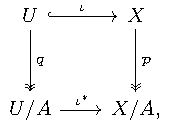
\includegraphics{figures/hw4-quotient-diagram}
\end{center}
it follows by Problem 4.4 (Theorem Q.2) that $\iota^*$ is
continuous. Alternatively, we note that $\iota^*\colon U/A\to
X/A$ is the inclusion map, and therefore, is continuous.
\\\\
(ii) We prove the following stronger but simple (to prove) result:
\begin{lemma}
Suppose $Y\subset X$ is open. The inclusion $\iota\colon Y\hookrightarrow X$ is
an open map.
\end{lemma}
\begin{proof}
\renewcommand\qedsymbol{$\clubsuit$}
Let $U$ be an open in $Y$. Then, by Lemma 16.2, $\iota(U)=U$ is open in
$X$. Thus $\iota$ is an open map.
\end{proof}
If we can show that $U/A$ is open in $X/A$, it follows from Lemma
12 that $\iota^*$ is an open map. Looking at the diagram in part
(i) above, the we have that
\[
\iota(q^{-1}(U/A))=\iota(U)=U=p^{-1}(U/A)
\]
is open in $X$, hence, by the definition of the quotient map,
$U/A$ is open in $X/A$. Thus, the map $\iota^*$ is open in
$X/A$.
\end{proof}
\newpage
\begin{problem}[G]
Let $X$ be a topological space satisfying the first countability
axiom (see the bottom of page 130 and the top of page 131). Let
$A\subset X$ and let $x\in\clsr{A}$. Prove that there is a
sequence in $A$ which converges to $x$ (see the top of page 131
for a hint).
\end{problem}
\begin{proof}
Suppose that $X$ satisfies the first countability axiom. Let
$x\in\clsr A$. We will construct a sequence $\left\{x_n\right\}$
which converges to $x$. Since $x$ is in the closure of $A$, for
every neighborhood $U$ of $x$ the intersection $U\cap A$ is
nonempty. In particular, since $X$ is first countable, there is a
countable collection $\left\{U_n\right\}$ of neighborhoods of $x$
with $U_n\cap A\neq\emptyset$ for all $n$. Now, define a nested
sequence of sets $V_1\supset V_2\supset\cdots\supset
V_n\supset\cdots$ where $V_n=\bigcap_{i=1}^n U_i$ and let $x_n\in
V_n\cap A$. (Note that $V_n$ is nonempty since it is a
neighborhood of $x$ so for some positive integer $N$ the
neighborhood $U_N\subset V_n$. Moreover $V_n\cap A$ is nonempty
since $V_n$ is a neighborhood of $x$ which is in the closure of
$A$.) We claim that the sequence we just created,
$\left\{x_n\right\}$, converges to $x$. Let $U$ be any neighborhood of
$x$. Then $U_N\subset U$ for some positive integer $N$. Hence
$x_n\in U$ for every $n\geq N$ (by construction). Thus, the
sequence $x_n\to
x$.
\end{proof}

%%% Local Variables:
%%% mode: latex
%%% TeX-master: "../MA571-HW-Current"
%%% End:
